\section{Conclusions}
\begin{figure*}
    \begin{minipage}[t]{0.32\textwidth}
        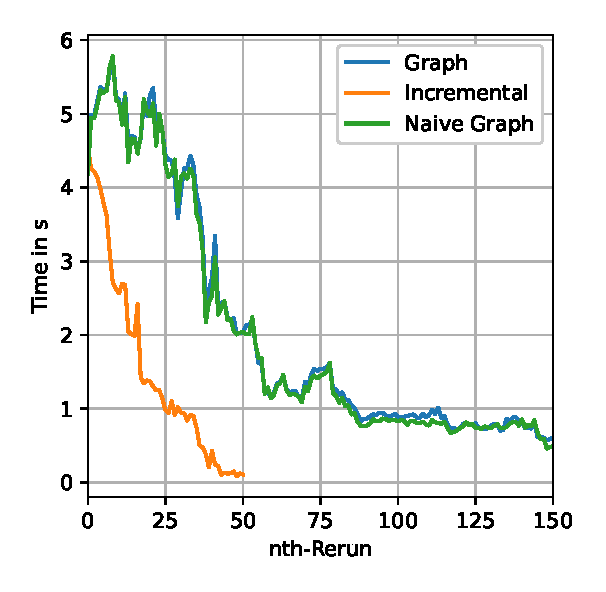
\includegraphics[width=1\textwidth]{benchmarking/sparse_rerun_cropped.eps}
        \caption{Sparse: Reruns}
        \label{fig:sparse_cropped}
    \end{minipage}
    \begin{minipage}[t]{0.32\textwidth}
        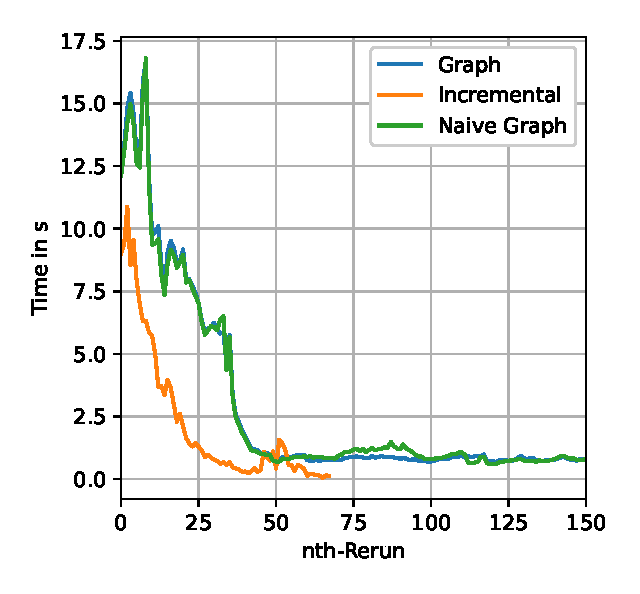
\includegraphics[width=1\textwidth]{benchmarking/medium_rerun_cropped.eps}
        \caption{Medium: Reruns}
        \label{fig:medium_cropped}
    \end{minipage}
    \begin{minipage}[t]{0.32\textwidth}
        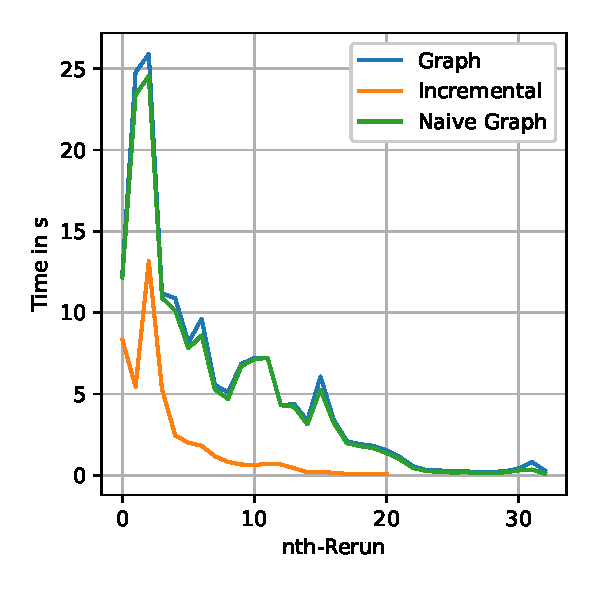
\includegraphics[width=1\textwidth]{benchmarking/dense_rerun_cropped.eps}
        \caption{Dense: Reruns}
        \label{fig:dense_cropped}
    \end{minipage}
\end{figure*}

As visible in Figure \ref{fig:sparse_cropped}, \ref{fig:medium_cropped} and \ref{fig:dense_cropped} our hypothesis, that the graph approach might have problems with an escalating window, did not hold true.

\begin{figure*}
	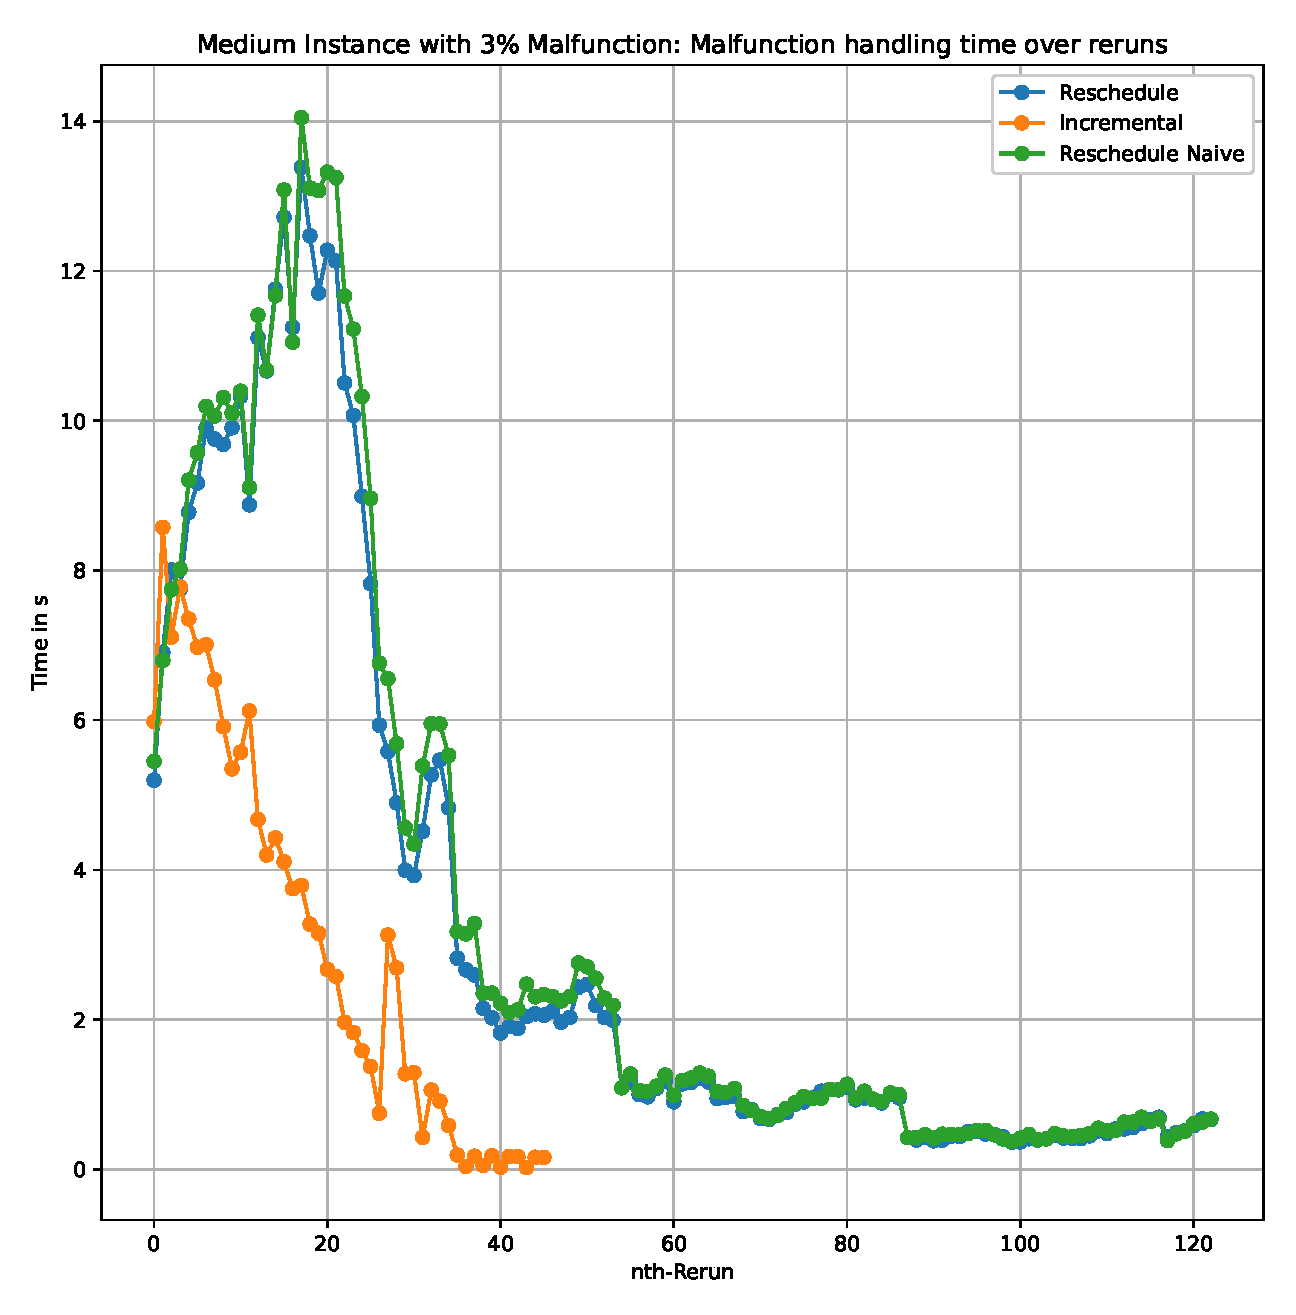
\includegraphics[width=1\textwidth]{benchmarking/medium_3_4_rerun_full.eps}
	\caption{A selected medium Instance, 3\% Malfunction}
	\label{fig:medium_instance}
\end{figure*}

As Figure \ref{fig:medium_instance} illustrates, the first reruns have a growing time consumption (in the example up to the 20th rerun), but after some trains have reached their goals, the rerun time decreases as does the window, due to fewer malfunctions. It is still not the most efficient solution, as the incremental approach illustrates, but the escalation is not as bad as expected.

The assumption, that the malfunction handling of the graph approach works worst for malfunction dense environments did not hold. The assumption was that more malfunctions, extend the computation window by too much, when using the worst case estimate (as in graph). Taking incremental as a comparison, one can see, that the graph approach performs better in the dense setting, thus refuting our assumption. We did not take into account, that more malfunctions also tend to approach the worst case, and thus improve the performance of the approach relatively.

Our assumption that the naive approach would perform worse than the graph approach did not hold. It seems, that computing the graph is similarly efficient as reading the graph from input, with most instances performing slightly better, if the graph is recomputed (naive).

But the assumption, of the incremental outperforming the other approaches did hold. It shows shorter runtimes over all instances, also requiring less reruns, as it's solutions always use the optimal horizon. The window is shrinking on every rerun and only extended if required. One can spot the reruns, where more timesteps were necessary, by looking at the peaks in Figure \ref{fig:medium_instance}.

\section{Fazit}
I out testing environment the hybrid approach of using the estimate and incrementing the timesteps, when required, outperformed the others on all instances. This illustrates the advantages and the ability of an incremental approach to build on and adapt previous knowledge and shows a problem for which such an approach is a good fit. An expansion on the incremental approach, would be, as the map does not change to pass the grounded map and train space, to new runs and only add new assumptions on a malfunction.

As a side benefit, incremental compute shorter paths (thus needing fewer reruns), as it finds timestep optimal solutions. Optimality, would be a good topic for further study, as enforcing optimality (e.g. trains arrive with as much time left as possible) might further reduce, the necessary window and quicken reruns.

Another idea, not thematized by this paper, is to use more resilient paths, which ensure a minimum distance between trains, enabling more reusing of previous paths, when reruns happen.  

Other than that, all ideas which limit grounding and solving are worth pursuing and applicable to Flatland as long as they are applicable to graph structures.
